\chapter{6 Questions With A Public CEO}

This lecture is an interview, but it is not loose. It has a strong internal order. We begin with authority and origin, move into a model of sales, then into mentor advice and humility, then into the most structured conceptual stretch of the lecture, namely White's picture of trauma and the brain, and finally back out into failure, bankruptcy, and daily self-repair. There is no blackboard mathematics here, but there is a clear mathematics of process: observation becomes offer, questions become tailored communication, trauma becomes dysregulation, and one kept promise becomes the basis for the next.

\section{A Public CEO and the Shape of a First Business}

The host frames Mark White as a public-company CEO whose business concerns brain health and the restoration of mental well-being. That opening matters because it tells us how the lecture wants to be read: not as motivational noise, but as advice backed by entrepreneurial experience, public responsibility, and a concrete domain.

The first real move is backward. White is asked what his first business was, and he answers without ornament: car detailing. The story then becomes quite precise. He is a valet parker in Houston during the late 1970s. Hotel guests leave their cars while they go inside for dinner. Armor All is new; the visual effect of cleaned wheels and treated tires is dramatic. White and the doorman notice that the customer's car is idle for exactly the length of time in which a visible improvement can be made. The customer's time is not additionally taxed; the customer's attention is captured at the return.

We can compress the entrepreneurial logic of the episode into a small causal formula:
\begin{equation}
\text{idle customer time}+\text{visible car improvement}+p_0 \to \text{first paying service},
\qquad p_0=20\text{ dollars}.
\end{equation}
The point of the story is not merely that White washed cars. It is that he identified a narrow market window, matched the service to that window, and chose an offer small enough to lower the threshold for a first yes.

It is worth writing the mechanism out explicitly.
\begin{enumerate}
\item The customer is already committed to spending time inside the hotel.
\item Hence the service can be offered without asking for extra customer time.
\item The result is immediately visible when the customer returns to the car.
\item A low first price makes the demonstration itself carry the sale.
\item The first demonstration then opens the way to repeat and expanded business.
\end{enumerate}
That last point matters. White does not stay at the one-shot hotel interaction. He begins picking up cars from offices, taking them home, detailing them carefully, and returning them improved. The first business is therefore not only a hustle; it is a miniature theory of entrepreneurial fit between circumstance, offer, and proof.

\section{Sales as Communication Rather Than Closing}

From the origin story the lecture pivots naturally into sales. The host asks for White's view of sales, given his years spent around brain and psychology language. White does mention classic names, Zig Ziglar and Tony Robbins, but he does so mainly in order to move past them. He does not deny the value of training; he redefines the center of gravity.

His claim is that his selling is not fundamentally about the theatrical close. It is about energy, confidence, communication, and a real affection for what he is talking about. In the notes we may write the structure this way:
\begin{align}
\text{ask questions} &\to \text{listen carefully} \to \text{tailor the message},\\
\text{tailored message} &\to \text{relevance} \to \text{engagement}.
\end{align}
And the supporting claim is equally compact:
\begin{equation}
\text{passion for the product}+\text{clear communication}
\to
\text{natural sales moment}.
\end{equation}

This is one of the lecture's strongest turns. White says that when he walks into a room, one of the first things he asks himself is why the room might say no. That is a strategic question, but it is also a moral question. It forces the speaker to begin not with self-expression but with resistance, need, and ignorance. One listens before one instructs.

The medical-professional example sharpens the point. White says that when he is in a room of perhaps thirty people, he may begin by asking how many medical professionals are present. Hands go up. The first move is then not to dominate the room, but to show humility. He does not pretend to know healthcare better than those who practice it. He offers a vision of a better system and tries to speak in a way that respects the actual knowledge already present in the audience.

So the lecture does not define sales as pressure. It defines sales as informed communication under the discipline of respect. The earlier car-detailing story now reveals itself as the first version of the same principle: the first sale worked because the offer was calibrated to the customer's actual situation, not because the pitch was loud.

\section{Mentor Advice, Money, and the Discipline of Humility}

The next question concerns the best advice White ever received from a mentor. The answer comes in two pieces, and both are corrective. The first is verbal: slow down, use fewer words, and remember that the people listening do not know the material as well as the speaker does. The correction is subtle. It is not a call to say less because less is fashionable; it is a call to say less because transmission fails when the speaker outruns the hearer.

The second piece is financial. White insists that money must be handled carefully, and that in the entrepreneurial life personal and professional spending easily bleed into one another. A good week in the business can intoxicate the owner. A few thousand dollars come in, and immediately one is in an expensive store or at an expensive restaurant acting as though a transient inflow were durable wealth.

The lecture does not present this as a bookkeeping theorem, but the logic is sharp enough to summarize:
\begin{equation}
\text{temporary revenue without restraint} \to \text{overconfidence in lifestyle},
\end{equation}
where the right-hand side is exactly what humility is meant to block.

White then names humility outright as one of the central traits of his professional life. He says he is confident and aggressive, but also tries to remain aware of what he does not know. This is not a sentimental ornament. It is the condition that keeps salesmanship from turning into bluff, and success from turning into self-deception.

The lecture briefly roughens in the transcript here, but the surviving line is still useful: White calls himself a talker. The chapter should preserve the tension. He is a talker, but the lecture has just defined the disciplined version of talking: fewer words, better calibration, and greater respect for the listener.

\section{Trauma, Regulation, and White's Two-System Picture of the Brain}

The interview now makes its largest turn. The host raises a difficult example, namely the case of Kanye West, the loss of his mother, and the question of how relational or emotional trauma can affect the brain without a visible head injury. This is the moment in the lecture where narrative pressure becomes conceptual pressure.

\subsection{Question \& Answer}

\paragraph{Question.} How can the loss of a relationship, or the loss of a loved one, produce something like serious mental instability even when there has been no physical blow to the head?

\paragraph{Answer.} White begins by broadening the definition of trauma. He does not restrict it to catastrophic physical injury. Instead, he treats trauma as any abnormal disturbance imposed on ordinary life. He then sorts it into three classes.

\begin{definition}
In White's vocabulary, trauma is not only a spectacular injury. It is any abnormal intrusion into the ordinary course of life experience, and he sorts it schematically into toxic, physical, and emotional forms.
\end{definition}

We may encode that classification as
\begin{equation}
T=\{T_{\mathrm{tox}},\,T_{\mathrm{phys}},\,T_{\mathrm{emo}}\},
\end{equation}
where \(T_{\mathrm{tox}}\) denotes toxic trauma, \(T_{\mathrm{phys}}\) physical trauma, and \(T_{\mathrm{emo}}\) emotional trauma.

White then introduces his central model of the brain. He says the brain has two systems, an electrical system and a chemical system, and that these two systems ``dance'' together in the ordinary conduct of life. In our notation:
\begin{equation}
B=(E,C),
\end{equation}
where \(E\) is the electrical side of regulation and \(C\) is the chemical side. Later in the interview White associates \(E\) with EEG and frequencies, and \(C\) with neurotransmitter language such as dopamine, serotonin, and acetylcholine.

The causal chain he proposes is then:
\begin{equation}
T \to R_{\mathrm{ff}} \to D_{\mathrm{post}},
\end{equation}
where \(R_{\mathrm{ff}}\) is the protective fight-or-flight response and \(D_{\mathrm{post}}\) is the lingering dysregulation that may remain after the immediate crisis has passed.

The logic is as follows.
\begin{enumerate}
\item Trauma arrives, whether toxic, physical, or emotional.
\item The brain activates a protective response in order to save the organism in the moment.
\item That protective response is useful in the crisis itself.
\item But once the trauma has passed, the system may fail to return cleanly to ordinary regulation.
\item What remains is a stressed or imbalanced state, which White associates with broader PTSD-like consequences.
\end{enumerate}

This is why White insists that PTSD should not be thought of as an exclusively military category. The phrase itself, in his reading, already says what is needed: after trauma, there is a stress disorder. A bad marriage, a bad employer, or the loss of a loved one can all fall under that broader description.

\begin{remark}
The notation in this section is a compact transcription of White's verbal model, not a formal derivation from neuroscience. The lecture gives us a causal picture, not a technical proof.
\end{remark}

Since no board figure survives for this lecture, we keep the reconstruction deliberately schematic:
\begin{figure}
\centering
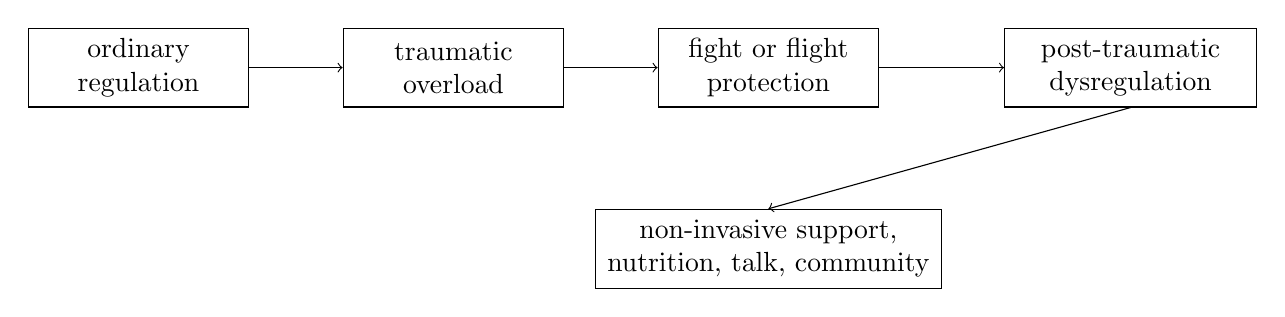
\begin{tikzpicture}
\node[draw, rectangle, minimum width=2.8cm, minimum height=1cm, align=center] (A) at (0,0) {ordinary\\ regulation};
\node[draw, rectangle, minimum width=2.8cm, minimum height=1cm, align=center] (B) at (4,0) {traumatic\\ overload};
\node[draw, rectangle, minimum width=2.8cm, minimum height=1cm, align=center] (C) at (8,0) {fight or flight\\ protection};
\node[draw, rectangle, minimum width=3.2cm, minimum height=1cm, align=center] (D) at (12.6,0) {post-traumatic\\ dysregulation};
\node[draw, rectangle, minimum width=4.4cm, minimum height=1cm, align=center] (Ebox) at (8,-2.3) {non-invasive support,\\ nutrition, talk, community};
\draw[->] (A.east) -- (B.west);
\draw[->] (B.east) -- (C.west);
\draw[->] (C.east) -- (D.west);
\draw[->] (D.south) -- (Ebox.north);
\end{tikzpicture}
\end{figure}

The treatment discussion follows the same picture. White says that a common medical response is trial-and-error chemical intervention: a patient presents with depression, loss of desire, or a collapsing marriage, and a drug is tried. He is careful to say, with all fairness to doctors and psychiatrists, that this becomes a guessing game. We should keep the force of the claim, but also its attribution. It is White's critique.

What he proposes instead is an order of response:
\begin{equation}
\text{non-invasive support} \to \text{gradual restoration of function}.
\end{equation}
And the order itself is concrete: non-invasive technologies, nutrition, talk or therapeutic conversation, friendship, spiritual community, and only then the patient work of recovery. The lecture presses this with an analogy to weight gain. One does not get into trouble overnight and one does not get out overnight. This becomes the bridge to the later section on habit and structure.

\section{Bankruptcy, Creditors, and the Measure of Accomplishment}

After the trauma section, the host pivots back to biography with a question that sounds at first like a request for triumph. What is White's greatest accomplishment? The answer refuses the expected glamour. It is not taking a company public. It is not the moment of money. It is getting up again after being broken by failure.

White states the thought almost as a grim aphorism: the worst thing is not never having money; it is having a lot of money, losing it, and then having none. This leads directly into the bankruptcy story. He recalls watching the work of his life being loaded into trucks and taken away. He names his bankruptcy attorney, Nelson Hemsley, and credits him with a decisive gift. The attorney offers a choice: pay me and disappear while I clean up your mess, or come with me to every meeting, every court appearance, every confrontation with the people who lost money because of your failure.

The educational structure is severe:
\begin{equation}
\text{loss} \to \text{accountability} \to \text{humility} \to \text{reconstruction}.
\end{equation}
White chooses the harder branch. He goes into rooms of people who hate him because they have lost money. He does not present this as a noble theatrical apology. He is more exact than that. He describes being in an apologetic space, surrendering what remains, and enduring the brutality of having a failed life-work divided and sold.

The payoff comes only on the far side. He says he became a new man. He gained respect for others, rebuilt family life, and learned humility in a form that no clean success could have taught. This is why the lecture's ethical center is not the public-company credential from the opening, but the bankruptcy courtroom from the middle. Success is redefined as the ability to face consequences without evasion.

\section{Structure, Small Wins, and a Daily Update Rule}

The final section of the lecture turns practical again. The host asks for White's best self-improvement advice, especially for the average modern man who is out of shape, overstimulated, and scattered. White answers with a single word: structure.

He then tells the story of a man named Haas, who gave him a program so simple that it nearly sounds insulting. Set the alarm for 8 a.m. Get out of bed. Make the bed. Shower. Be ready by 9. Eat lunch at noon. Eat dinner at six. Begin preparing for sleep at a fixed hour. The program is not impressive in content. It is impressive in discipline. The point is not heroism. The point is to be successful at something.

We may turn White's idea into a minimal update rule. Let \(a_n\in\{0,1\}\) record whether the one promised act on day \(n\) is completed, and let \(s_n\) count the number of kept promises to oneself up to that day. Then
\begin{equation}
s_{n+1}=s_n+a_n.
\end{equation}
This is elementary arithmetic, but it captures the lecture exactly. White is not asking for a grand reinvention. He is asking for accumulative evidence that one can do what one says.

The cycle can also be written schematically as
\begin{align}
\text{one promised act} &\to \text{completion} \to \text{reflection},\\
&\to \text{confidence} \to \text{next promised act}.
\end{align}

A worked example makes the logic plain.
\begin{enumerate}
\item On day \(n\), one promise is chosen: get out of bed at 8 a.m.\ and make the bed.
\item If the promise is kept, then \(a_n=1\) and \(s_{n+1}=s_n+1\).
\item The day is then closed not with fantasy, but with reflection: I did what I said I would do.
\item Only after that proof has been repeated does one enlarge the program.
\end{enumerate}

This is why White is suspicious of the usual all-at-once self-improvement fantasy. One declares that today is the day, makes a long list, gets through the first fragment of it, fails, feels shame, and collapses back into distraction. The lecture names the pattern with unusual sharpness: Netflix, chips, and surrender. White's alternative is not romantic. It is small, repetitive, and therefore hard in the correct way.

The advice closes with a demand for honesty. Each person has an Achilles heel. It may be sugar, alcohol, marijuana, a bad marriage, cruelty, or some other destabilizing habit. One must identify it clearly and then choose a bounded action that can actually be kept. Even something as small as saying hello to everybody and smiling for a day counts, provided it is real and completed.

\section{Summary}

This interview proceeds by layers. First we are shown the first business, where observation, timing, and a low-friction offer produce a first sale. Then we are given a theory of sales as communication rather than pressure. Then humility and money discipline are introduced as correctives. From there the lecture turns to its most structured conceptual section, White's model of trauma, the brain, and the slow work of restoring regulation. Finally, it returns to biography and to daily practice: face failure directly, accept accountability, and rebuild by structure and small completed acts.

What makes the lecture worth preserving is precisely this order. It does not begin with abstraction. It begins with a parked car, moves through a speaking voice, passes through trauma and bankruptcy, and ends with an alarm clock and a made bed. That is its real mathematics: one causal step at a time, taken in the order in which a life can actually bear them.